% ============================================================
%  <<TITLE>> -- ACM Computing Surveys (CSUR) format, acmart/acmsmall.
%  Compiler: pdfLaTeX (latexmk -pdf). Replace every <<PLACEHOLDER>>.
% ============================================================
\PassOptionsToPackage{svgnames,dvipsnames}{xcolor} % acmart loads xcolor; set options first
\documentclass[acmsmall,screen,nonacm]{acmart}

\acmJournal{CSUR}
\acmYear{<<YEAR>>}\acmVolume{1}\acmNumber{1}\acmArticle{1}\acmMonth{1}
\settopmatter{authorsperrow=3}

% ---- taxonomy figure packages ----
\usepackage{forest}
\useforestlibrary{edges}   % forked edges
\usepackage{tikz}
\usetikzlibrary{arrows.meta,positioning,fit,backgrounds,shapes.geometric,calc}
\usepackage{pifont}
\usepackage{longtable}
\usepackage{placeins}      % \FloatBarrier

% coloured yes/no/partial/na marks for every comparison table
\newcommand{\yy}{\textcolor{ForestGreen}{\ding{52}}}
\newcommand{\nn}{\textcolor{BrickRed}{\ding{56}}}
\newcommand{\dm}{\textcolor{gray!65}{\textbf{--}}}
\newcommand{\pp}{\textcolor{orange!90!black}{\textbf{\textasciitilde}}}

% coloured category labels (rename per topic's branches)
\newcommand{\tcatA}{\textcolor{cat-code!55!black}{\textsf{\textbf{<<branchA>>}}}}
\newcommand{\tcatB}{\textcolor{cat-vla!45!black}{\textsf{\textbf{<<branchB>>}}}}
% eval-domain labels
\newcommand{\dreal}{\textcolor{ForestGreen}{\textsf{real}}}
\newcommand{\dsim}{\textcolor{RoyalBlue}{\textsf{sim}}}
\newcommand{\dgame}{\textcolor{Purple}{\textsf{game}}}
\newcommand{\dtext}{\textcolor{gray!70}{\textsf{text}}}

% ============================================================
%  Shared taxonomy style: forked-edge forest (grow=east, reversed),
%  rounded
%  rectangles, per-category colour blocks.  Content colours are our
%  six robot-learning domains.
% ============================================================

% ---- draw + root ----
\definecolor{hidden-draw}{RGB}{40,40,40}
\definecolor{tx-root}{HTML}{D1D5DB}

% ---- per-domain category (darker) / leaf (lighter) fills ----
\definecolor{cat-code}{HTML}{93C5FD}\definecolor{leaf-code}{HTML}{DBEAFE}   % §3.1 blue
\definecolor{cat-vla}{HTML}{5EEAD4}\definecolor{leaf-vla}{HTML}{CCFBF1}     % §3.2 teal
\definecolor{cat-rew}{HTML}{FDBA74}\definecolor{leaf-rew}{HTML}{FEEBC8}     % §3.3 orange
\definecolor{cat-skill}{HTML}{C4B5FD}\definecolor{leaf-skill}{HTML}{EDE9FE} % §3.4 purple
\definecolor{cat-trans}{HTML}{F9A8D4}\definecolor{leaf-trans}{HTML}{FCE7F3} % §3.5 pink
\definecolor{cat-bench}{HTML}{86EFAC}\definecolor{leaf-bench}{HTML}{DCFCE7} % §3.6 green

% ---- per-sub-section palette (deep-dive figures: one colour per sub-section) ----
\definecolor{secA}{HTML}{93C5FD}\definecolor{secAl}{HTML}{DBEAFE} % blue
\definecolor{secB}{HTML}{5EEAD4}\definecolor{secBl}{HTML}{CCFBF1} % teal
\definecolor{secC}{HTML}{86EFAC}\definecolor{secCl}{HTML}{DCFCE7} % green
\definecolor{secD}{HTML}{FCD34D}\definecolor{secDl}{HTML}{FEF3C7} % amber
\definecolor{secE}{HTML}{FCA5A5}\definecolor{secEl}{HTML}{FEE2E2} % red (the gap)
\definecolor{secF}{HTML}{C4B5FD}\definecolor{secFl}{HTML}{EDE9FE} % purple
\definecolor{secG}{HTML}{F9A8D4}\definecolor{secGl}{HTML}{FCE7F3} % pink

% ---- the forest style, applied to every tree via default preamble ----
\forestset{
  default preamble={
    forked edges,
    for tree={
      grow=east,
      reversed=true,
      anchor=base west,
      parent anchor=east,
      child anchor=west,
      base=center,
      font=\large,
      rectangle,
      draw=hidden-draw,
      rounded corners,
      align=center,
      text centered,
      minimum width=5em,
      edge+={darkgray, line width=1pt},
      s sep=3pt,
      inner xsep=2pt,
      inner ysep=3pt,
      line width=0.8pt,
      ver/.style={rotate=90, child anchor=north, parent anchor=south, anchor=center},
      % per-level widths applied per node (reliable inside for tree)
      if level=1{text width=19em, font=\normalsize}{},
      if level=2{text width=33em, font=\normalsize}{},
    },
  },
}
   % shared forest style + palette (topic-agnostic)

\begin{document}

\title{<<SHORT TITLE>>}
\subtitle{<<SUBTITLE: A Survey of ... >>}

\author{<<AUTHOR1>>}
\affiliation{\institution{<<INST1>>}\country{<<C1>>}}
% ... more authors ...
\renewcommand{\shortauthors}{<<Lastname>> et al.}

\input{sections/0_abstract}

\begin{CCSXML}
<ccs2012>
   <concept><concept_id><<CCS_ID>></concept_id>
   <concept_desc><<CCS_DESC>></concept_desc>
   <concept_significance>500</concept_significance></concept>
</ccs2012>
\end{CCSXML}
\ccsdesc[500]{<<CCS_DESC>>}
\keywords{<<kw1, kw2, ..., survey>>}
\maketitle

\section{Introduction}
\label{sec:intro}

Two paradigms now dominate robot learning. \emph{Vision-language-action} (VLA)
models predict actions from frozen weights; \emph{code-as-policy} agents instead
write executable programs and improve them from experience~\citep{codeaspolicies,aspire}.
This survey is organized around that fault line.

\paragraph{Why now: the skill stack.}
The app store for robot skills has arrived---Unitree UniStore ships one-tap,
cross-model motion downloads~\citep{unistore2026}. But every skill in it is
\emph{canned playback}: the least-capable point on our map. The skill stack has
three layers---\textbf{(1) Build} (how skills are created, \S\ref{sec:taxonomy}--\S\ref{sec:techniques}),
\textbf{(2) Distribute} (marketplaces and hubs), and \textbf{(3) Adapt} (on-device
self-improvement, \S\ref{sec:code}). UniStore is layer~2 over static layer-1 skills;
the promised value---``adjust grip per fruit so nothing bruises''---lives in layer~3,
which no shipped skill does today.

\paragraph{Contributions.}
(i) a taxonomy of robot-learning techniques organized by \emph{weights vs.\ skills}
(\S\ref{sec:taxonomy}); (ii) a deep-dive arranging code-as-policy by \emph{degree of
self-improvement} and isolating the un-surveyed \S3.1.5 cell (\S\ref{sec:code});
(iii) a companion map of the ``skills'' pole (\S\ref{sec:skill}); and (iv) an
open-problems agenda for the emerging skill economy (\S\ref{sec:open}).

\paragraph{Related surveys.}
Table~\ref{tab:survey_compare} contrasts the topical coverage of the closest surveys with
ours, and Table~\ref{tab:surveys} places them on a timeline. Within \emph{ACM Computing
Surveys} the nearest are on world models, embodied intelligence, and language-model
navigation, and beyond it a cluster covers vision-language-action models and foundation models
for manipulation---but none organises code-as-policy by degree of self-improvement or names
the \S3.1.5 cell.
% Table — coverage of related surveys vs. ours.
\begin{table}[t]
\centering
\footnotesize
\renewcommand{\arraystretch}{1.25}
\begin{tabular}{@{}p{0.24\textwidth}c c *{6}{c}@{}}
\toprule
\textbf{Survey} & \textbf{Venue} & \textbf{Yr}
  & \tweights{} & \tcode{} & \tskill{} & \treward{}
  & \textcolor{secE!55!black}{\textbf{Self-impr.}} & \textcolor{cat-bench!45!black}{\textbf{Economy}}\\
\midrule
World Models~\cite{survey_worldmodels}          & CSUR  & 2025 & \pp & \nn & \nn & \nn & \nn & \nn\\
Embodied Intelligence~\cite{survey_embodiedintel}& CSUR  & 2025 & \pp & \nn & \pp & \nn & \nn & \nn\\
Navigation via FLM~\cite{survey_navigation}      & CSUR  & 2026 & \pp & \pp & \nn & \nn & \nn & \nn\\
VLA for Embodied AI~\cite{survey_vla}            & arXiv & 2024 & \yy & \nn & \nn & \nn & \nn & \nn\\
Large-VLM VLA~\cite{survey_vlmvla}               & arXiv & 2025 & \yy & \nn & \nn & \pp & \nn & \nn\\
Embodied Learning~\cite{survey_embodiedlearn}    & MIR   & 2025 & \pp & \nn & \pp & \pp & \nn & \nn\\
FM for Manipulation~\cite{survey_fmrobot}        & arXiv & 2024 & \yy & \pp & \pp & \pp & \nn & \nn\\
\midrule
\textbf{Ours (\emph{Weights or Skills?})}        & ---   & 2026 & \yy & \yy & \yy & \yy & \yy & \yy\\
\bottomrule
\end{tabular}
\caption{Topical coverage of the closest related surveys versus ours.
\yy\ covered, \pp\ partial/mentioned, \nn\ not covered. Columns: \tweights{} (VLA/weights),
\tcode{} (code-as-policy), \tskill{} (skill libraries), \treward{} (reward synthesis),
\textbf{Self-impr.}\ (organised by \emph{degree of self-improvement}, incl.\ the \S3.1.5 cell),
\textbf{Economy} (the robot skill marketplace). Only this survey covers the last two axes.
CSUR = ACM Computing Surveys; MIR = Machine Intelligence Research.}
\label{tab:survey_compare}
\end{table}

% Table 1 — related surveys as a colored TikZ timeline (year axis, one marker each).
\begin{table}[t]
\centering
\resizebox{\columnwidth}{!}{%
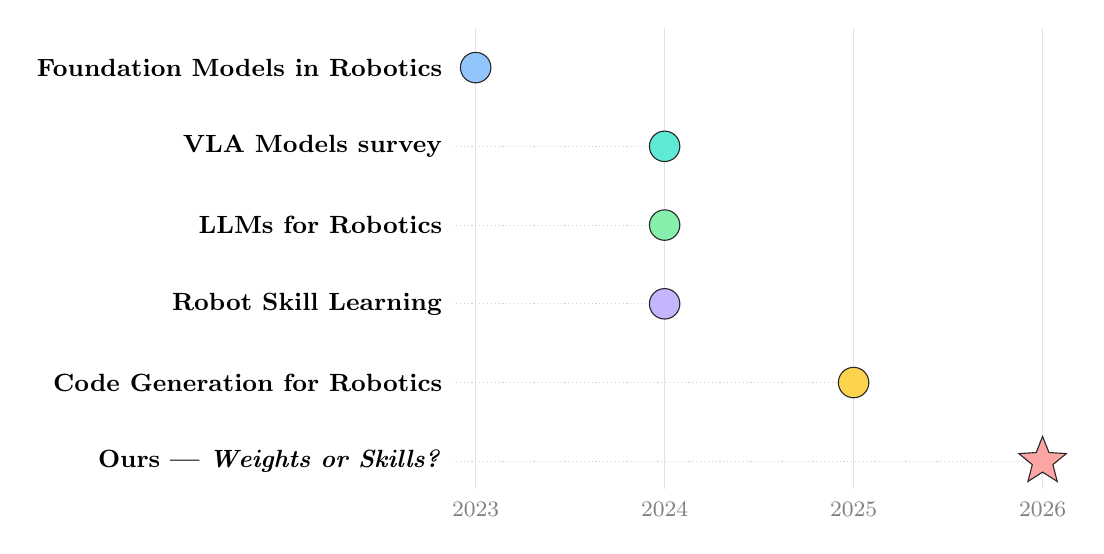
\begin{tikzpicture}[font=\small]
  % year gridlines + labels
  \foreach \x/\yr in {0/2023, 2.4/2024, 4.8/2025, 7.2/2026}{
    \draw[gray!22] (\x,-0.35) -- (\x,5.5);
    \node[gray, font=\footnotesize, below] at (\x,-0.4) {\yr};
  }
  % rows: dotted leader + name (left) + colored marker at its year
  \draw[gray!35, densely dotted] (-0.25,5) -- (0,5);
  \node[anchor=east] at (-0.3,5) {\textbf{Foundation Models in Robotics}};
  \filldraw[fill=secA, draw=hidden-draw] (0,5) circle (5.5pt);

  \draw[gray!35, densely dotted] (-0.25,4) -- (2.4,4);
  \node[anchor=east] at (-0.3,4) {\textbf{VLA Models survey}};
  \filldraw[fill=secB, draw=hidden-draw] (2.4,4) circle (5.5pt);

  \draw[gray!35, densely dotted] (-0.25,3) -- (2.4,3);
  \node[anchor=east] at (-0.3,3) {\textbf{LLMs for Robotics}};
  \filldraw[fill=secC, draw=hidden-draw] (2.4,3) circle (5.5pt);

  \draw[gray!35, densely dotted] (-0.25,2) -- (2.4,2);
  \node[anchor=east] at (-0.3,2) {\textbf{Robot Skill Learning}};
  \filldraw[fill=secF, draw=hidden-draw] (2.4,2) circle (5.5pt);

  \draw[gray!35, densely dotted] (-0.25,1) -- (4.8,1);
  \node[anchor=east] at (-0.3,1) {\textbf{Code Generation for Robotics}};
  \filldraw[fill=secD, draw=hidden-draw] (4.8,1) circle (5.5pt);

  \draw[gray!35, densely dotted] (-0.25,0) -- (7.2,0);
  \node[anchor=east] at (-0.3,0) {\textbf{Ours --- \emph{Weights or Skills?}}};
  \node[star, star points=5, star point ratio=2.3, fill=secE, draw=hidden-draw,
        minimum size=18pt, inner sep=0] at (7.2,0) {};
\end{tikzpicture}%
}
\caption{Related surveys on a timeline. Prior surveys (2023--2025) each cover part of the
landscape---foundation models, VLA policies, LLM planning, skill acquisition, code
generation---but none organizes code-as-policy by \emph{degree of self-improvement}.
\textbf{Ours} ($\star$, 2026) isolates the feedback\,+\,memory\,+\,search cell (\S3.1.5)
that ASPIRE occupies.}
\label{tab:surveys}
\end{table}

\FloatBarrier
          % scope+contributions para; inputs tab_survey_compare,
                                  % fig_taxonomy_main, fig_survey_timeline; \FloatBarrier
\section{A Taxonomy of Robot-Learning Techniques}
\label{sec:taxonomy}

Figure~\ref{fig:taxonomy_main} organises the field into six branches. The dividing
question is \emph{what ships}: frozen weights (\S\ref{sec:vla}) or executable skills
(\S\ref{sec:code}). We tag mechanisms by \textbf{F}eedback, \textbf{S}earch, and
\textbf{M}emory throughout.

Table~\ref{tab:compare_main} compares all systems in the map on what each \emph{ships}, where
it is evaluated, and whether it improves from its own experience.
\input{tables/tab_compare_main}

\subsection{Survey methodology: how the corpus was built}
\label{sec:method}

Figure~\ref{fig:prisma} summarises the corpus construction in the PRISMA~2020
style~\citep{prisma2020}. The corpus was assembled in two passes over a January~2016 to
July~2026 window. First, the 77 taxonomy systems were curated by \emph{seeding and
snowballing}: for each of the six branches we started from its landmark systems and chased
citations forward and backward until new candidates stopped appearing. Second, the 225-work
landscape corpus (Table~\ref{tab:landscape}) was gathered by five \emph{structured web-search
sweeps}, one per area cluster: (i) generalist and vision-language-action policies, imitation
and diffusion policies; (ii) language-model planning, task-and-motion planning, reward and data
synthesis; (iii) skill discovery, hierarchical reinforcement learning, and world models;
(iv) manipulation, dexterity, sim-to-real, locomotion, and benchmarks; and (v) representation
learning, offline reinforcement learning, navigation, and tactile sensing. Each sweep queried
the open web with area-specific search strings of the form ``\emph{<system or family name>
robot learning arXiv}'' and ``\emph{<area> survey/benchmark/dataset}'' over arXiv, the ACM
Digital Library, IEEE Xplore, Google Scholar, and venue proceedings pages (CoRL, RSS, ICRA,
IROS, NeurIPS, ICML, ICLR, CVPR).

\emph{Inclusion} required a work to (a) concern how an embodied agent's skill or policy is
authored, learned, transferred, evaluated, or distributed, and (b) carry verifiable metadata:
exact title, first author, year, and an arXiv identifier or DOI, each confirmed against the
source. \emph{Exclusion} removed pure perception, navigation, and locomotion work with no
bearing on skill authoring (retained only in the landscape appendix where it anchors an area),
works whose metadata could not be verified, and duplicates, detected by both bibliographic key
and arXiv identifier. Every reference in this survey passed the verification step; candidates
that failed it were discarded at harvest time, and we report that their count was not logged
rather than estimate it. Included systems were then mapped onto the taxonomy of
Figure~\ref{fig:taxonomy_main} by the mechanism definitions of Table~\ref{tab:defs}.

% PRISMA-2020-style corpus-construction flow with recorded counts (see methodology subsection).
% Upright TWO-COLUMN design: two identification streams side by side, each stage's exclusions folded
% inline (red italic) rather than as separate side-boxes. Two boxes across fit the text width, so
% \resizebox scales the picture UP -> figure text renders at/above body size. Do NOT re-add separate
% side exclusion boxes (3 boxes across overflows the column and shrinks the font below body size).
\begin{figure}[t]
\centering
\resizebox{\textwidth}{!}{%
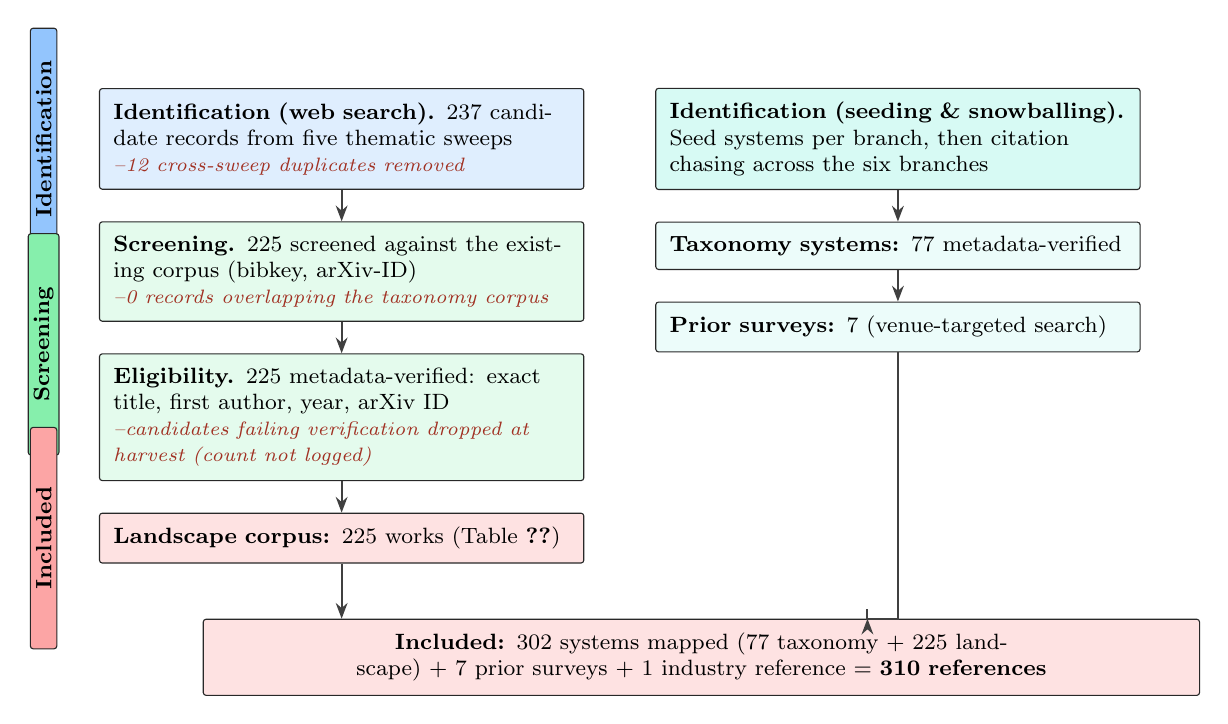
\begin{tikzpicture}[
  font=\footnotesize,
  box/.style={draw=hidden-draw, rounded corners=1pt, align=left, inner sep=5pt,
              text width=16.5em, fill=white},
  ex/.style={font=\scriptsize\itshape, text=BrickRed!85!black},
  bar/.style={draw=hidden-draw, rounded corners=1pt, inner sep=2pt, rotate=90,
              anchor=center, align=center, font=\footnotesize\bfseries, minimum width=8em},
  ar/.style={-{Stealth[length=2mm]}, darkgray, line width=0.7pt},
  node distance=4mm and 9mm,
]
% ---- left column: structured web-search stream (exclusions inline, red italic) ----
\node[box, fill=secA!30] (L1)
  {\textbf{Identification (web search).} 237 candidate records from five thematic sweeps\\
   {\scriptsize\itshape\color{BrickRed!85!black} --12 cross-sweep duplicates removed}};
\node[box, fill=secC!22, below=of L1] (L2)
  {\textbf{Screening.} 225 screened against the existing corpus (bibkey, arXiv-ID)\\
   {\scriptsize\itshape\color{BrickRed!85!black} --0 records overlapping the taxonomy corpus}};
\node[box, fill=secC!22, below=of L2] (L3)
  {\textbf{Eligibility.} 225 metadata-verified: exact title, first author, year, arXiv ID\\
   {\scriptsize\itshape\color{BrickRed!85!black} --candidates failing verification dropped at harvest (count not logged)}};
\node[box, fill=secEl, below=of L3] (L4)
  {\textbf{Landscape corpus:} 225 works (Table~\ref{tab:landscape})};
% ---- right column: seed-and-snowball curation ----
\node[box, fill=secB!25, right=9mm of L1] (R1)
  {\textbf{Identification (seeding \& snowballing).} Seed systems per branch, then citation
   chasing across the six branches};
\node[box, fill=secB!12, below=of R1] (R2)
  {\textbf{Taxonomy systems:} 77 metadata-verified};
\node[box, fill=secB!12, below=of R2] (R3)
  {\textbf{Prior surveys:} 7 (venue-targeted search)};
% ---- merged included box ----
\node[box, fill=secEl, below=7mm of L4, xshift=13em, text width=35em, align=center] (INC)
  {\textbf{Included:} 302 systems mapped (77 taxonomy $+$ 225 landscape) $+$ 7 prior surveys
   $+$ 1 industry reference $=$ \textbf{310 references}};
% ---- arrows ----
\draw[ar] (L1) -- (L2); \draw[ar] (L2) -- (L3); \draw[ar] (L3) -- (L4);
\draw[ar] (R1) -- (R2); \draw[ar] (R2) -- (R3);
\draw[ar] (L4.south) -- (L4.south |- INC.north);
\draw[ar] (R3.south) |- ([xshift=6em]INC.north) -- ([xshift=6em]INC.north |- INC.north);
% ---- stage bars ----
\node[bar, fill=secA] at ($(L1.west)+(-2em,0)$) {Identification};
\node[bar, fill=secC] at ($(L2.west)!0.5!(L3.west)+(-2em,0)$) {Screening};
\node[bar, fill=secE] at ($(L4.west)+(-2em,0)$) {Included};
\end{tikzpicture}}
\caption{\textbf{Corpus construction} in the PRISMA 2020 style~\citep{prisma2020}. The left column
is the web-search stream behind the landscape corpus (Table~\ref{tab:landscape}), with recorded
counts and inline exclusions (red) at each stage; the right column is the seed-and-snowball
curation behind the taxonomy corpus (Figure~\ref{fig:taxonomy_main}). Both streams feed the
included set. Candidates whose metadata could not be verified were discarded at harvest time; their
count was not logged, which we state rather than estimate (\S\ref{sec:method}).}
\Description{A PRISMA 2020 style flow diagram with two identification columns. The left column
(structured web search) shows 237 candidate records, minus 12 duplicates, screened to 225 with zero
taxonomy overlap, and 225 metadata-verified records forming the landscape corpus; exclusions are
noted inline, including a note that candidates failing verification were dropped with their count
not logged. The right column (seed-and-snowball curation) yields 77 taxonomy systems and 7 prior
surveys. Both columns feed an included box of 302 systems and 310 total references. Side bars mark
the Identification, Screening, and Included stages.}
\label{fig:prisma}
\end{figure}

       % inputs tab_compare_main
\section{The Technique Families}
\label{sec:techniques}

We now examine each of the six branches of the taxonomy (Figure~\ref{fig:taxonomy_main}) in
turn. We begin with the code-as-policy camp (\S\ref{sec:code})---the focus of this survey and
the only family we organise by \emph{degree of self-improvement}---and then survey the
weights-based (\S\ref{sec:vla}), reward-synthesis (\S\ref{sec:reward}), skill-library
(\S\ref{sec:skill}), transfer (\S\ref{sec:transfer}), and benchmark (\S\ref{sec:bench})
families that surround it.
     % one \input per branch section below
% ... sections/3_<deepdive>.tex (rung membership conditions; tab_definitions; fig_architectures)
% ... sections/4..8 per branch; 9_open_problems; limitations; future_work; 10_conclusion

\bibliographystyle{ACM-Reference-Format}
\bibliography{refs}

% Appendices FOLLOW the references (ACM convention); fresh page.
\clearpage
% Appendix: comprehensive landscape table situating the 77 taxonomy systems within 200+ works.
\appendix
\section{The Broader Robot-Learning Landscape}
\label{sec:landscape}

The taxonomy of Figure~\ref{fig:taxonomy_main} foregrounds 77 systems chosen to populate a single
analytical axis, weights versus skills, rather than to enumerate the field. To situate those systems
within the wider research landscape, and to make the survey's coverage inspectable at a glance,
Table~\ref{tab:landscape} catalogues a further set of representative works: end-to-end and generalist
policies, imitation and diffusion policies, language-model planning and task-and-motion planning,
reward and data synthesis, unsupervised skill discovery and hierarchical reinforcement learning, world
models and model-based control, representation learning and offline reinforcement learning,
manipulation, dexterity, and locomotion, and the datasets, benchmarks, and simulators that support
them. Together with the 77 systems detailed in the main text
(Tables~\ref{tab:compare_main}--\ref{tab:compare_34}), the works surveyed number more than three
hundred. The list is representative rather than exhaustive; each entry is a real, individually
citeable paper, grouped by area and ordered by year.

% Comparison matrix of 200+ robot-learning works. AUTO-GENERATED; do not hand-edit.
{\scriptsize
\setlength{\tabcolsep}{4pt}
\renewcommand{\arraystretch}{1.1}
\begin{longtable}{@{}p{0.27\textwidth} c l l c l c@{}}
\caption{\textbf{The broader robot-learning landscape: 225 representative works, compared on six axes.} Beyond the 77 systems placed in the taxonomy (Figure~\ref{fig:taxonomy_main}, Tables~\ref{tab:compare_main}--\ref{tab:compare_34}), this table catalogues the wider field, grouped into eleven areas and sub-grouped by family. Columns: \textbf{Year}, \textbf{Ships} (what the method contributes), \textbf{Learn} (primary learning signal: IL, RL, offline-RL, LLM, self-sup., model-based), \textbf{Eval} (\dreal/\dsim/\dgame/offline), \textbf{Embod.} (embodiment), and run-time \textbf{S.I.} (self-improvement: \yy\ yes, \pp\ partial, \nn\ no). A \dm\ marks not-applicable or unverified. Every entry is a real, individually citeable paper.}\label{tab:landscape}\\
\toprule
\textbf{System / work} & \textbf{Year} & \textbf{Ships} & \textbf{Learn} & \textbf{Eval} & \textbf{Embod.} & \textbf{S.I.}\\
\midrule
\endfirsthead
\multicolumn{7}{@{}l}{\scriptsize\emph{Table~\ref{tab:landscape} (continued)}}\\
\toprule
\textbf{System / work} & \textbf{Year} & \textbf{Ships} & \textbf{Learn} & \textbf{Eval} & \textbf{Embod.} & \textbf{S.I.}\\
\midrule
\endhead
\bottomrule
\endlastfoot
\multicolumn{7}{@{}l}{\rule{0pt}{2.6ex}\textbf{\textsf{End-to-end \& generalist policies}}~\textcolor{gray}{(28)}}\\[1pt]
\multicolumn{7}{@{}l}{\hspace{0.6em}\emph{Vision-language-action}}\\
\hspace{0.6em}\textbf{3D-VLA}~\cite{vla3d} & 2024 & \textsf{world-model} & \textsf{LLM} & \dsim & \textsf{arm} & \nn\\
\hspace{0.6em}\textbf{ECoT}~\cite{ecot} & 2024 & \textsf{policy} & \textsf{IL} & \dreal & \textsf{arm} & \nn\\
\hspace{0.6em}\textbf{LLaRA}~\cite{llara} & 2024 & \textsf{policy} & \textsf{LLM} & \dsim & \textsf{arm} & \nn\\
\hspace{0.6em}\textbf{ManipLLM}~\cite{manipllm} & 2024 & \textsf{policy} & \textsf{LLM} & \dsim & \textsf{arm} & \nn\\
\hspace{0.6em}\textbf{RoboMamba}~\cite{robomamba} & 2024 & \textsf{policy} & \textsf{LLM} & \dsim & \textsf{arm} & \nn\\
\hspace{0.6em}\textbf{RoboPoint}~\cite{robopoint} & 2024 & \textsf{plan} & \textsf{LLM} & \dreal & \textsf{multi} & \nn\\
\hspace{0.6em}\textbf{TinyVLA}~\cite{tinyvla} & 2024 & \textsf{policy} & \textsf{IL} & \dreal & \textsf{arm} & \nn\\
\hspace{0.6em}\textbf{TraceVLA}~\cite{tracevla} & 2024 & \textsf{policy} & \textsf{IL} & \dsim & \textsf{arm} & \nn\\
\hspace{0.6em}\textbf{DexVLA}~\cite{dexvla} & 2025 & \textsf{policy} & \textsf{IL} & \dreal & \textsf{multi} & \nn\\
\hspace{0.6em}\textbf{FAST}~\cite{fast} & 2025 & \textsf{repr} & \textsf{IL} & \dreal & \textsf{arm} & \nn\\
\hspace{0.6em}\textbf{OpenVLA-OFT}~\cite{openvlaoft} & 2025 & \textsf{policy} & \textsf{IL} & \dsim & \textsf{arm} & \nn\\
\multicolumn{7}{@{}l}{\hspace{0.6em}\emph{Generalist / multi-task}}\\
\hspace{0.6em}\textbf{QT-Opt}~\cite{qtopt} & 2018 & \textsf{policy} & \textsf{RL} & \dreal & \textsf{arm} & \pp\\
\hspace{0.6em}\textbf{MT-Opt}~\cite{mtopt} & 2021 & \textsf{policy} & \textsf{RL} & \dreal & \textsf{arm} & \pp\\
\hspace{0.6em}\textbf{Gato}~\cite{gato} & 2022 & \textsf{policy} & \textsf{IL} & \dsim & \textsf{multi} & \nn\\
\hspace{0.6em}\textbf{PaLM-E}~\cite{palme} & 2023 & \textsf{plan} & \textsf{LLM} & \dreal & \textsf{multi} & \nn\\
\hspace{0.6em}\textbf{Q-Transformer}~\cite{qtransformer} & 2023 & \textsf{policy} & \textsf{offline-RL} & \dreal & \textsf{arm} & \nn\\
\hspace{0.6em}\textbf{UniPi}~\cite{unipi} & 2023 & \textsf{policy} & \textsf{model-based} & \dsim & \textsf{arm} & \nn\\
\hspace{0.6em}\textbf{VIMA}~\cite{vima} & 2023 & \textsf{policy} & \textsf{IL} & \dsim & \textsf{arm} & \nn\\
\hspace{0.6em}\textbf{GR-2}~\cite{gr2} & 2024 & \textsf{policy} & \textsf{IL} & \dreal & \textsf{arm} & \nn\\
\hspace{0.6em}\textbf{LEO}~\cite{leo} & 2024 & \textsf{policy} & \textsf{LLM} & \dsim & \textsf{multi} & \nn\\
\hspace{0.6em}\textbf{Magma}~\cite{magma} & 2025 & \textsf{weights} & \textsf{LLM} & \dsim & \textsf{arm} & \nn\\
\multicolumn{7}{@{}l}{\hspace{0.6em}\emph{Video / action pretraining}}\\
\hspace{0.6em}\textbf{ATM}~\cite{atm} & 2024 & \textsf{policy} & \textsf{self-sup} & \dsim & \textsf{arm} & \nn\\
\hspace{0.6em}\textbf{GR-1}~\cite{gr1} & 2024 & \textsf{policy} & \textsf{IL} & \dsim & \textsf{arm} & \nn\\
\hspace{0.6em}\textbf{HPT}~\cite{hpt} & 2024 & \textsf{repr} & \textsf{IL} & \dsim & \textsf{multi} & \nn\\
\hspace{0.6em}\textbf{VPP}~\cite{vpp} & 2024 & \textsf{policy} & \textsf{IL} & \dsim & \textsf{arm} & \nn\\
\hspace{0.6em}\textbf{Cosmos}~\cite{cosmos} & 2025 & \textsf{world-model} & \textsf{self-sup} & \dm & \dm & \nn\\
\hspace{0.6em}\textbf{LAPA}~\cite{lapa} & 2025 & \textsf{policy} & \textsf{self-sup} & \dsim & \textsf{arm} & \nn\\
\hspace{0.6em}\textbf{Seer}~\cite{seer} & 2025 & \textsf{policy} & \textsf{IL} & \dsim & \textsf{arm} & \nn\\
\addlinespace[2pt]
\multicolumn{7}{@{}l}{\rule{0pt}{2.6ex}\textbf{\textsf{Imitation \& diffusion policies}}~\textcolor{gray}{(21)}}\\[1pt]
\multicolumn{7}{@{}l}{\hspace{0.6em}\emph{Imitation learning}}\\
\hspace{0.6em}\textbf{BC-Z}~\cite{bcz} & 2021 & \textsf{policy} & \textsf{IL} & \dreal & \textsf{arm} & \nn\\
\hspace{0.6em}\textbf{Implicit BC}~\cite{ibc} & 2021 & \textsf{policy} & \textsf{IL} & \dsim & \textsf{arm} & \nn\\
\hspace{0.6em}\textbf{robomimic}~\cite{robomimic} & 2021 & \textsf{bench} & \textsf{IL} & \dsim & \textsf{arm} & \nn\\
\hspace{0.6em}\textbf{PerAct}~\cite{peract} & 2022 & \textsf{policy} & \textsf{IL} & \dsim & \textsf{arm} & \nn\\
\hspace{0.6em}\textbf{ACT/ALOHA}~\cite{act} & 2023 & \textsf{policy} & \textsf{IL} & \dreal & \textsf{arm} & \nn\\
\hspace{0.6em}\textbf{MimicGen}~\cite{mimicgen} & 2023 & \textsf{data} & \textsf{IL} & \dsim & \textsf{arm} & \nn\\
\hspace{0.6em}\textbf{RVT}~\cite{rvt} & 2023 & \textsf{policy} & \textsf{IL} & \dsim & \textsf{arm} & \nn\\
\hspace{0.6em}\textbf{Mobile ALOHA}~\cite{mobilealoha} & 2024 & \textsf{policy} & \textsf{IL} & \dreal & \textsf{mobile} & \nn\\
\hspace{0.6em}\textbf{RoboAgent}~\cite{roboagent} & 2024 & \textsf{policy} & \textsf{IL} & \dreal & \textsf{arm} & \nn\\
\hspace{0.6em}\textbf{RVT-2}~\cite{rvt2} & 2024 & \textsf{policy} & \textsf{IL} & \dsim & \textsf{arm} & \nn\\
\hspace{0.6em}\textbf{UMI}~\cite{umi} & 2024 & \textsf{data} & \textsf{IL} & \dreal & \textsf{arm} & \nn\\
\multicolumn{7}{@{}l}{\hspace{0.6em}\emph{Diffusion policies}}\\
\hspace{0.6em}\textbf{Diffuser}~\cite{diffuser} & 2022 & \textsf{plan} & \textsf{model-based} & \textcolor{gray!70}{\textsf{offline}} & \dm & \nn\\
\hspace{0.6em}\textbf{BESO}~\cite{beso} & 2023 & \textsf{policy} & \textsf{IL} & \dsim & \textsf{arm} & \nn\\
\hspace{0.6em}\textbf{Decision Diffuser}~\cite{decisiondiffuser} & 2023 & \textsf{policy} & \textsf{offline-RL} & \textcolor{gray!70}{\textsf{offline}} & \dm & \nn\\
\hspace{0.6em}\textbf{Diffusion Policy}~\cite{diffusionpolicy} & 2023 & \textsf{policy} & \textsf{IL} & \dsim & \textsf{arm} & \nn\\
\hspace{0.6em}\textbf{3D Diffuser Actor}~\cite{diffuseractor3d} & 2024 & \textsf{policy} & \textsf{IL} & \dsim & \textsf{arm} & \nn\\
\hspace{0.6em}\textbf{DP3}~\cite{dp3} & 2024 & \textsf{policy} & \textsf{IL} & \dsim & \textsf{arm} & \nn\\
\hspace{0.6em}\textbf{Equivariant Diffusion Policy}~\cite{equidiff} & 2024 & \textsf{policy} & \textsf{IL} & \dsim & \textsf{arm} & \nn\\
\hspace{0.6em}\textbf{MDT}~\cite{mdt} & 2024 & \textsf{policy} & \textsf{IL} & \dsim & \textsf{arm} & \nn\\
\hspace{0.6em}\textbf{RDT-1B}~\cite{rdt1b} & 2024 & \textsf{weights} & \textsf{IL} & \dreal & \textsf{arm} & \nn\\
\hspace{0.6em}\textbf{SuSIE}~\cite{susie} & 2024 & \textsf{policy} & \textsf{IL} & \dsim & \textsf{arm} & \nn\\
\addlinespace[2pt]
\multicolumn{7}{@{}l}{\rule{0pt}{2.6ex}\textbf{\textsf{LLM/VLM planning \& task-and-motion}}~\textcolor{gray}{(30)}}\\[1pt]
\multicolumn{7}{@{}l}{\hspace{0.6em}\emph{LLM task planning}}\\
\hspace{0.6em}\textbf{COWP}~\cite{cowp} & 2022 & \textsf{plan} & \textsf{LLM} & \dsim & \textsf{mobile} & \pp\\
\hspace{0.6em}\textbf{ReAct}~\cite{react} & 2022 & \textsf{plan} & \textsf{LLM} & \dgame & \dm & \pp\\
\hspace{0.6em}\textbf{SayCan}~\cite{saycan} & 2022 & \textsf{plan} & \textsf{LLM} & \dreal & \textsf{mobile} & \nn\\
\hspace{0.6em}\textbf{Socratic Models}~\cite{socraticmodels} & 2022 & \textsf{plan} & \textsf{LLM} & \dreal & \textsf{arm} & \nn\\
\hspace{0.6em}\textbf{Zero-Shot Planners}~\cite{zeroshotplanners} & 2022 & \textsf{plan} & \textsf{LLM} & \dsim & \dm & \nn\\
\hspace{0.6em}\textbf{DEPS}~\cite{deps} & 2023 & \textsf{plan} & \textsf{LLM} & \dgame & \dm & \pp\\
\hspace{0.6em}\textbf{GLAM}~\cite{glam} & 2023 & \textsf{policy} & \textsf{RL} & \dgame & \dm & \nn\\
\hspace{0.6em}\textbf{Grounded Decoding}~\cite{grounddecoding} & 2023 & \textsf{plan} & \textsf{LLM} & \dreal & \textsf{mobile} & \nn\\
\hspace{0.6em}\textbf{ISR-LLM}~\cite{isrllm} & 2023 & \textsf{plan} & \textsf{LLM} & \dsim & \dm & \pp\\
\hspace{0.6em}\textbf{ITP}~\cite{interactivetaskplanning} & 2023 & \textsf{plan} & \textsf{LLM} & \dreal & \textsf{arm} & \pp\\
\hspace{0.6em}\textbf{KnowNo}~\cite{knowno} & 2023 & \textsf{plan} & \textsf{LLM} & \dreal & \textsf{arm} & \nn\\
\hspace{0.6em}\textbf{LLM-Planner}~\cite{llmplanner} & 2023 & \textsf{plan} & \textsf{LLM} & \dsim & \textsf{mobile} & \pp\\
\hspace{0.6em}\textbf{Reflexion}~\cite{reflexion} & 2023 & \textsf{plan} & \textsf{LLM} & \dgame & \dm & \yy\\
\hspace{0.6em}\textbf{RoCo}~\cite{roco} & 2023 & \textsf{plan} & \textsf{LLM} & \dsim & \textsf{multi} & \pp\\
\hspace{0.6em}\textbf{SayPlan}~\cite{sayplan} & 2023 & \textsf{plan} & \textsf{LLM} & \dreal & \textsf{mobile} & \pp\\
\hspace{0.6em}\textbf{Self-Refine}~\cite{selfrefine} & 2023 & \textsf{plan} & \textsf{LLM} & \dm & \dm & \yy\\
\hspace{0.6em}\textbf{SMART-LLM}~\cite{smartllm} & 2023 & \textsf{plan} & \textsf{LLM} & \dsim & \textsf{multi} & \nn\\
\hspace{0.6em}\textbf{Tree-Planner}~\cite{treeplanner} & 2023 & \textsf{plan} & \textsf{LLM} & \dsim & \dm & \pp\\
\hspace{0.6em}\textbf{ReAd}~\cite{readmarl} & 2024 & \textsf{plan} & \textsf{LLM} & \dsim & \textsf{multi} & \pp\\
\multicolumn{7}{@{}l}{\hspace{0.6em}\emph{LLM task-and-motion}}\\
\hspace{0.6em}\textbf{AutoTAMP}~\cite{autotamp} & 2023 & \textsf{plan} & \textsf{LLM} & \dsim & \dm & \pp\\
\hspace{0.6em}\textbf{Lang2LTL}~\cite{lang2ltl} & 2023 & \textsf{plan} & \textsf{LLM} & \dreal & \textsf{mobile} & \nn\\
\hspace{0.6em}\textbf{LLM+P}~\cite{llmp} & 2023 & \textsf{plan} & \textsf{LLM} & \dm & \dm & \nn\\
\hspace{0.6em}\textbf{LLM-GROP}~\cite{llmgrop} & 2023 & \textsf{plan} & \textsf{LLM} & \dsim & \textsf{mobile} & \nn\\
\hspace{0.6em}\textbf{NL2TL}~\cite{nl2tl} & 2023 & \textsf{plan} & \textsf{LLM} & \textcolor{gray!70}{\textsf{offline}} & \dm & \nn\\
\hspace{0.6em}\textbf{DELTA}~\cite{delta} & 2024 & \textsf{plan} & \textsf{LLM} & \dsim & \textsf{mobile} & \nn\\
\hspace{0.6em}\textbf{LLM3}~\cite{llm3} & 2024 & \textsf{plan} & \textsf{LLM} & \dsim & \textsf{arm} & \pp\\
\multicolumn{7}{@{}l}{\hspace{0.6em}\emph{Code / prompt as policy}}\\
\hspace{0.6em}\textbf{LM Traj Generators}~\cite{zeroshottraj} & 2023 & \textsf{plan} & \textsf{LLM} & \dreal & \textsf{arm} & \pp\\
\hspace{0.6em}\textbf{MOKA}~\cite{moka} & 2024 & \textsf{plan} & \textsf{LLM} & \dreal & \textsf{arm} & \nn\\
\hspace{0.6em}\textbf{PIVOT}~\cite{pivot} & 2024 & \textsf{plan} & \textsf{LLM} & \dreal & \textsf{mobile} & \pp\\
\hspace{0.6em}\textbf{ReKep}~\cite{rekep} & 2024 & \textsf{code} & \textsf{LLM} & \dreal & \textsf{arm} & \pp\\
\addlinespace[2pt]
\multicolumn{7}{@{}l}{\rule{0pt}{2.6ex}\textbf{\textsf{LLM reward synthesis \& data generation}}~\textcolor{gray}{(17)}}\\[1pt]
\multicolumn{7}{@{}l}{\hspace{0.6em}\emph{LLM reward synthesis}}\\
\hspace{0.6em}\textbf{ELLM}~\cite{ellm} & 2023 & \textsf{reward} & \textsf{RL} & \dgame & \dm & \nn\\
\hspace{0.6em}\textbf{LAMP}~\cite{lamp} & 2023 & \textsf{reward} & \textsf{RL} & \dsim & \textsf{arm} & \nn\\
\hspace{0.6em}\textbf{Motif}~\cite{motif} & 2023 & \textsf{reward} & \textsf{RL} & \dgame & \dm & \nn\\
\hspace{0.6em}\textbf{Read and Reap}~\cite{readreap} & 2023 & \textsf{reward} & \textsf{RL} & \dgame & \dm & \nn\\
\hspace{0.6em}\textbf{VLM-RM}~\cite{vlmrm} & 2023 & \textsf{reward} & \textsf{RL} & \dsim & \textsf{humanoid} & \nn\\
\hspace{0.6em}\textbf{Code as Reward}~\cite{codeasreward} & 2024 & \textsf{reward} & \textsf{RL} & \dsim & \dm & \nn\\
\hspace{0.6em}\textbf{RL-VLM-F}~\cite{rlvlmf} & 2024 & \textsf{reward} & \textsf{RL} & \dsim & \textsf{arm} & \nn\\
\multicolumn{7}{@{}l}{\hspace{0.6em}\emph{Generative data / augmentation}}\\
\hspace{0.6em}\textbf{CACTI}~\cite{cacti} & 2022 & \textsf{data} & \textsf{IL} & \dreal & \textsf{arm} & \nn\\
\hspace{0.6em}\textbf{DIAL}~\cite{dial} & 2022 & \textsf{data} & \textsf{IL} & \dreal & \textsf{mobile} & \nn\\
\hspace{0.6em}\textbf{GenAug}~\cite{genaug} & 2023 & \textsf{data} & \textsf{IL} & \dreal & \textsf{arm} & \nn\\
\hspace{0.6em}\textbf{GenSim}~\cite{gensim} & 2023 & \textsf{data} & \textsf{IL} & \dsim & \textsf{arm} & \nn\\
\hspace{0.6em}\textbf{ROSIE}~\cite{rosie} & 2023 & \textsf{data} & \textsf{IL} & \dreal & \textsf{mobile} & \nn\\
\hspace{0.6em}\textbf{Scaling Up Distilling Down}~\cite{scalingup} & 2023 & \textsf{policy} & \textsf{IL} & \dreal & \textsf{arm} & \nn\\
\hspace{0.6em}\textbf{BBSEA}~\cite{bbsea} & 2024 & \textsf{skill} & \textsf{IL} & \dsim & \textsf{arm} & \pp\\
\hspace{0.6em}\textbf{DexMimicGen}~\cite{dexmimicgen} & 2024 & \textsf{data} & \textsf{IL} & \dsim & \textsf{humanoid} & \nn\\
\hspace{0.6em}\textbf{GenSim2}~\cite{gensim2} & 2024 & \textsf{data} & \textsf{IL} & \dsim & \textsf{arm} & \nn\\
\hspace{0.6em}\textbf{RoboDreamer}~\cite{robodreamer} & 2024 & \textsf{world-model} & \textsf{model-based} & \dm & \textsf{arm} & \nn\\
\addlinespace[2pt]
\multicolumn{7}{@{}l}{\rule{0pt}{2.6ex}\textbf{\textsf{Unsupervised skill discovery \& hierarchical RL}}~\textcolor{gray}{(25)}}\\[1pt]
\multicolumn{7}{@{}l}{\hspace{0.6em}\emph{Unsupervised skill discovery}}\\
\hspace{0.6em}\textbf{VIC}~\cite{vic} & 2016 & \textsf{skill} & \textsf{RL} & \dsim & \dm & \nn\\
\hspace{0.6em}\textbf{Eigenoption}~\cite{eigenoption} & 2018 & \textsf{skill} & \textsf{RL} & \dgame & \dm & \nn\\
\hspace{0.6em}\textbf{VALOR}~\cite{valor} & 2018 & \textsf{skill} & \textsf{RL} & \dsim & \dm & \nn\\
\hspace{0.6em}\textbf{EDL}~\cite{edl} & 2020 & \textsf{skill} & \textsf{RL} & \dsim & \dm & \nn\\
\hspace{0.6em}\textbf{VISR}~\cite{visr} & 2020 & \textsf{skill} & \textsf{RL} & \dgame & \dm & \pp\\
\hspace{0.6em}\textbf{APS}~\cite{aps} & 2021 & \textsf{skill} & \textsf{RL} & \dgame & \dm & \nn\\
\hspace{0.6em}\textbf{APT}~\cite{apt} & 2021 & \textsf{skill} & \textsf{RL} & \dgame & \dm & \nn\\
\hspace{0.6em}\textbf{ProtoRL}~\cite{protorl} & 2021 & \textsf{repr} & \textsf{self-sup} & \dsim & \dm & \nn\\
\hspace{0.6em}\textbf{WURL}~\cite{wurl} & 2022 & \textsf{skill} & \textsf{RL} & \dsim & \dm & \nn\\
\hspace{0.6em}\textbf{BeCL}~\cite{becl} & 2023 & \textsf{skill} & \textsf{RL} & \dsim & \dm & \nn\\
\hspace{0.6em}\textbf{Choreographer}~\cite{choreographer} & 2023 & \textsf{skill} & \textsf{model-based} & \dsim & \dm & \nn\\
\hspace{0.6em}\textbf{CSD}~\cite{csd} & 2023 & \textsf{skill} & \textsf{RL} & \dsim & \textsf{multi} & \nn\\
\hspace{0.6em}\textbf{DGPO}~\cite{dgpo} & 2024 & \textsf{skill} & \textsf{RL} & \dsim & \dm & \nn\\
\multicolumn{7}{@{}l}{\hspace{0.6em}\emph{Hierarchical / option RL}}\\
\hspace{0.6em}\textbf{h-DQN}~\cite{hdqn} & 2016 & \textsf{policy} & \textsf{RL} & \dgame & \dm & \nn\\
\hspace{0.6em}\textbf{FeUdal Networks}~\cite{feudalnet} & 2017 & \textsf{policy} & \textsf{RL} & \dgame & \dm & \nn\\
\hspace{0.6em}\textbf{Option-Critic}~\cite{optioncritic} & 2017 & \textsf{skill} & \textsf{RL} & \dgame & \dm & \nn\\
\hspace{0.6em}\textbf{SNN4HRL}~\cite{snn4hrl} & 2017 & \textsf{skill} & \textsf{RL} & \dsim & \textsf{multi} & \nn\\
\hspace{0.6em}\textbf{HIRO}~\cite{hiro} & 2018 & \textsf{policy} & \textsf{RL} & \dsim & \textsf{legged} & \nn\\
\hspace{0.6em}\textbf{MLSH}~\cite{mlsh} & 2018 & \textsf{skill} & \textsf{RL} & \dsim & \textsf{multi} & \pp\\
\hspace{0.6em}\textbf{HAC}~\cite{hac} & 2019 & \textsf{policy} & \textsf{RL} & \dsim & \textsf{arm} & \nn\\
\hspace{0.6em}\textbf{MCP}~\cite{mcp} & 2019 & \textsf{skill} & \textsf{RL} & \dsim & \textsf{humanoid} & \nn\\
\hspace{0.6em}\textbf{NPMP}~\cite{npmp} & 2019 & \textsf{skill} & \textsf{IL} & \dsim & \textsf{humanoid} & \nn\\
\hspace{0.6em}\textbf{Relay Policy Learning}~\cite{relaypolicy} & 2019 & \textsf{policy} & \textsf{IL} & \dsim & \textsf{arm} & \nn\\
\hspace{0.6em}\textbf{HIDIO}~\cite{hidio} & 2021 & \textsf{skill} & \textsf{RL} & \dsim & \textsf{multi} & \nn\\
\hspace{0.6em}\textbf{Director}~\cite{director} & 2022 & \textsf{policy} & \textsf{model-based} & \dsim & \dm & \nn\\
\addlinespace[2pt]
\multicolumn{7}{@{}l}{\rule{0pt}{2.6ex}\textbf{\textsf{World models \& model-based RL}}~\textcolor{gray}{(24)}}\\[1pt]
\multicolumn{7}{@{}l}{\hspace{0.6em}\emph{World models}}\\
\hspace{0.6em}\textbf{World Models}~\cite{worldmodels} & 2018 & \textsf{world-model} & \textsf{model-based} & \dgame & \dm & \nn\\
\hspace{0.6em}\textbf{PlaNet}~\cite{planet} & 2019 & \textsf{world-model} & \textsf{model-based} & \dsim & \dm & \nn\\
\hspace{0.6em}\textbf{Dreamer}~\cite{dreamer} & 2020 & \textsf{world-model} & \textsf{model-based} & \dsim & \dm & \nn\\
\hspace{0.6em}\textbf{DreamerV2}~\cite{dreamerv2} & 2021 & \textsf{world-model} & \textsf{model-based} & \dgame & \dm & \nn\\
\hspace{0.6em}\textbf{DayDreamer}~\cite{daydreamer} & 2022 & \textsf{world-model} & \textsf{model-based} & \dreal & \textsf{multi} & \yy\\
\hspace{0.6em}\textbf{Iso-Dream}~\cite{isodream} & 2022 & \textsf{world-model} & \textsf{model-based} & \dsim & \dm & \nn\\
\hspace{0.6em}\textbf{MWM}~\cite{mwm} & 2022 & \textsf{world-model} & \textsf{model-based} & \dsim & \textsf{arm} & \nn\\
\hspace{0.6em}\textbf{TransDreamer}~\cite{transdreamer} & 2022 & \textsf{world-model} & \textsf{model-based} & \dgame & \dm & \nn\\
\hspace{0.6em}\textbf{DreamerV3}~\cite{dreamerv3} & 2023 & \textsf{world-model} & \textsf{model-based} & \dgame & \dm & \nn\\
\hspace{0.6em}\textbf{IRIS}~\cite{iris} & 2023 & \textsf{world-model} & \textsf{model-based} & \dgame & \dm & \nn\\
\hspace{0.6em}\textbf{STORM}~\cite{storm} & 2023 & \textsf{world-model} & \textsf{model-based} & \dgame & \dm & \nn\\
\hspace{0.6em}\textbf{SWIM}~\cite{swim} & 2023 & \textsf{world-model} & \textsf{model-based} & \dreal & \textsf{arm} & \nn\\
\hspace{0.6em}\textbf{TWM}~\cite{twm} & 2023 & \textsf{world-model} & \textsf{model-based} & \dgame & \dm & \nn\\
\hspace{0.6em}\textbf{DIAMOND}~\cite{diamond} & 2024 & \textsf{world-model} & \textsf{model-based} & \dgame & \dm & \nn\\
\hspace{0.6em}\textbf{Genie}~\cite{genie} & 2024 & \textsf{world-model} & \textsf{self-sup} & \dgame & \dm & \nn\\
\hspace{0.6em}\textbf{UniSim}~\cite{unisim} & 2024 & \textsf{world-model} & \textsf{self-sup} & \dreal & \textsf{arm} & \nn\\
\multicolumn{7}{@{}l}{\hspace{0.6em}\emph{Model-based RL}}\\
\hspace{0.6em}\textbf{PETS}~\cite{pets} & 2018 & \textsf{world-model} & \textsf{model-based} & \dsim & \dm & \nn\\
\hspace{0.6em}\textbf{MBPO}~\cite{mbpo} & 2019 & \textsf{policy} & \textsf{model-based} & \dsim & \dm & \nn\\
\hspace{0.6em}\textbf{MuZero}~\cite{muzero} & 2020 & \textsf{world-model} & \textsf{model-based} & \dgame & \dm & \nn\\
\hspace{0.6em}\textbf{SimPLe}~\cite{simple} & 2020 & \textsf{world-model} & \textsf{model-based} & \dgame & \dm & \nn\\
\hspace{0.6em}\textbf{SLAC}~\cite{slac} & 2020 & \textsf{repr} & \textsf{RL} & \dsim & \dm & \nn\\
\hspace{0.6em}\textbf{EfficientZero}~\cite{efficientzero} & 2021 & \textsf{world-model} & \textsf{model-based} & \dgame & \dm & \nn\\
\hspace{0.6em}\textbf{TD-MPC}~\cite{tdmpc} & 2022 & \textsf{world-model} & \textsf{model-based} & \dsim & \dm & \nn\\
\hspace{0.6em}\textbf{TD-MPC2}~\cite{tdmpc2} & 2024 & \textsf{world-model} & \textsf{model-based} & \dsim & \textsf{multi} & \nn\\
\addlinespace[2pt]
\multicolumn{7}{@{}l}{\rule{0pt}{2.6ex}\textbf{\textsf{Representation learning \& offline RL}}~\textcolor{gray}{(17)}}\\[1pt]
\multicolumn{7}{@{}l}{\hspace{0.6em}\emph{Visual representation learning}}\\
\hspace{0.6em}\textbf{MVP}~\cite{mvp} & 2022 & \textsf{repr} & \textsf{self-sup} & \dsim & \textsf{arm} & \nn\\
\hspace{0.6em}\textbf{PVR}~\cite{pvr} & 2022 & \textsf{repr} & \textsf{self-sup} & \dsim & \textsf{multi} & \nn\\
\hspace{0.6em}\textbf{R3M}~\cite{r3m} & 2022 & \textsf{repr} & \textsf{self-sup} & \dsim & \textsf{arm} & \nn\\
\hspace{0.6em}\textbf{LIV}~\cite{liv} & 2023 & \textsf{reward} & \textsf{self-sup} & \dreal & \textsf{arm} & \nn\\
\hspace{0.6em}\textbf{VC-1}~\cite{vc1} & 2023 & \textsf{repr} & \textsf{self-sup} & \dsim & \textsf{multi} & \nn\\
\hspace{0.6em}\textbf{VIP}~\cite{vip} & 2023 & \textsf{reward} & \textsf{self-sup} & \dreal & \textsf{arm} & \nn\\
\hspace{0.6em}\textbf{Voltron}~\cite{voltron} & 2023 & \textsf{repr} & \textsf{self-sup} & \dsim & \textsf{arm} & \nn\\
\hspace{0.6em}\textbf{Theia}~\cite{theia} & 2024 & \textsf{repr} & \textsf{self-sup} & \dsim & \textsf{arm} & \nn\\
\multicolumn{7}{@{}l}{\hspace{0.6em}\emph{Offline RL}}\\
\hspace{0.6em}\textbf{BCQ}~\cite{bcq} & 2019 & \textsf{policy} & \textsf{offline-RL} & \textcolor{gray!70}{\textsf{offline}} & \dm & \nn\\
\hspace{0.6em}\textbf{AWAC}~\cite{awac} & 2020 & \textsf{policy} & \textsf{offline-RL} & \textcolor{gray!70}{\textsf{offline}} & \dm & \pp\\
\hspace{0.6em}\textbf{CQL}~\cite{cql} & 2020 & \textsf{policy} & \textsf{offline-RL} & \textcolor{gray!70}{\textsf{offline}} & \dm & \nn\\
\hspace{0.6em}\textbf{Decision Transformer}~\cite{decisiontransformer} & 2021 & \textsf{policy} & \textsf{offline-RL} & \textcolor{gray!70}{\textsf{offline}} & \dm & \nn\\
\hspace{0.6em}\textbf{TD3+BC}~\cite{td3bc} & 2021 & \textsf{policy} & \textsf{offline-RL} & \textcolor{gray!70}{\textsf{offline}} & \dm & \nn\\
\hspace{0.6em}\textbf{Trajectory Transformer}~\cite{trajectorytransformer} & 2021 & \textsf{policy} & \textsf{offline-RL} & \textcolor{gray!70}{\textsf{offline}} & \dm & \nn\\
\hspace{0.6em}\textbf{IQL}~\cite{iql} & 2022 & \textsf{policy} & \textsf{offline-RL} & \textcolor{gray!70}{\textsf{offline}} & \dm & \nn\\
\hspace{0.6em}\textbf{Cal-QL}~\cite{calql} & 2023 & \textsf{policy} & \textsf{offline-RL} & \textcolor{gray!70}{\textsf{offline}} & \dm & \pp\\
\hspace{0.6em}\textbf{Diffusion-QL}~\cite{diffusionql} & 2023 & \textsf{policy} & \textsf{offline-RL} & \textcolor{gray!70}{\textsf{offline}} & \dm & \nn\\
\addlinespace[2pt]
\multicolumn{7}{@{}l}{\rule{0pt}{2.6ex}\textbf{\textsf{Manipulation, dexterity \& sim-to-real}}~\textcolor{gray}{(16)}}\\[1pt]
\multicolumn{7}{@{}l}{\hspace{0.6em}\emph{Manipulation / grasping}}\\
\hspace{0.6em}\textbf{Dex-Net 2.0}~\cite{dexnet2} & 2017 & \textsf{policy} & \dm & \dreal & \textsf{arm} & \nn\\
\hspace{0.6em}\textbf{GraspNet-1Billion}~\cite{graspnet1b} & 2020 & \textsf{bench} & \dm & \dreal & \textsf{arm} & \nn\\
\hspace{0.6em}\textbf{Transporter Nets}~\cite{transporter} & 2020 & \textsf{policy} & \textsf{IL} & \dsim & \textsf{arm} & \nn\\
\hspace{0.6em}\textbf{CLIPort}~\cite{cliport} & 2021 & \textsf{policy} & \textsf{IL} & \dsim & \textsf{arm} & \nn\\
\hspace{0.6em}\textbf{Contact-GraspNet}~\cite{contactgraspnet} & 2021 & \textsf{code} & \dm & \dreal & \textsf{arm} & \nn\\
\hspace{0.6em}\textbf{AnyGrasp}~\cite{anygrasp} & 2023 & \textsf{code} & \dm & \dreal & \textsf{arm} & \nn\\
\multicolumn{7}{@{}l}{\hspace{0.6em}\emph{Dexterous / in-hand}}\\
\hspace{0.6em}\textbf{Dactyl}~\cite{dactyl} & 2018 & \textsf{policy} & \textsf{RL} & \dreal & \textsf{hand} & \pp\\
\hspace{0.6em}\textbf{DAPG}~\cite{dapg} & 2018 & \textsf{policy} & \textsf{RL} & \dsim & \textsf{hand} & \nn\\
\hspace{0.6em}\textbf{Rubiks Cube Hand}~\cite{rubikscube} & 2019 & \textsf{policy} & \textsf{RL} & \dreal & \textsf{hand} & \pp\\
\hspace{0.6em}\textbf{DexPilot}~\cite{dexpilot} & 2020 & \textsf{code} & \dm & \dreal & \textsf{hand} & \nn\\
\hspace{0.6em}\textbf{Visual Dexterity}~\cite{visualdexterity} & 2023 & \textsf{policy} & \textsf{RL} & \dreal & \textsf{hand} & \nn\\
\multicolumn{7}{@{}l}{\hspace{0.6em}\emph{Sim-to-real transfer}}\\
\hspace{0.6em}\textbf{CAD2RL}~\cite{cad2rl} & 2017 & \textsf{policy} & \textsf{RL} & \dreal & \textsf{mobile} & \nn\\
\hspace{0.6em}\textbf{Domain Randomization}~\cite{domainrand} & 2017 & \textsf{code} & \dm & \dreal & \textsf{arm} & \nn\\
\hspace{0.6em}\textbf{Dynamics Randomization}~\cite{dynrand} & 2018 & \textsf{policy} & \textsf{RL} & \dreal & \textsf{arm} & \pp\\
\hspace{0.6em}\textbf{RCAN}~\cite{rcan} & 2019 & \textsf{policy} & \textsf{RL} & \dreal & \textsf{arm} & \nn\\
\hspace{0.6em}\textbf{SimOpt}~\cite{simopt} & 2019 & \textsf{policy} & \textsf{RL} & \dreal & \textsf{arm} & \pp\\
\addlinespace[2pt]
\multicolumn{7}{@{}l}{\rule{0pt}{2.6ex}\textbf{\textsf{Locomotion \& humanoid control}}~\textcolor{gray}{(16)}}\\[1pt]
\multicolumn{7}{@{}l}{\hspace{0.6em}\emph{Legged locomotion}}\\
\hspace{0.6em}\textbf{ANYmal}~\cite{anymal} & 2019 & \textsf{policy} & \textsf{RL} & \dreal & \textsf{legged} & \nn\\
\hspace{0.6em}\textbf{Quadruped Terrain}~\cite{quadterrain} & 2020 & \textsf{policy} & \textsf{RL} & \dreal & \textsf{legged} & \pp\\
\hspace{0.6em}\textbf{Legged Gym}~\cite{walkminutes} & 2021 & \textsf{code} & \textsf{RL} & \dreal & \textsf{legged} & \nn\\
\hspace{0.6em}\textbf{RMA}~\cite{rma} & 2021 & \textsf{policy} & \textsf{RL} & \dreal & \textsf{legged} & \pp\\
\hspace{0.6em}\textbf{Egocentric Locomotion}~\cite{egoloco} & 2022 & \textsf{policy} & \textsf{RL} & \dreal & \textsf{legged} & \pp\\
\hspace{0.6em}\textbf{Perceptive Locomotion}~\cite{perceptiveloco} & 2022 & \textsf{policy} & \textsf{RL} & \dreal & \textsf{legged} & \pp\\
\hspace{0.6em}\textbf{Walk These Ways}~\cite{walktheseways} & 2022 & \textsf{policy} & \textsf{RL} & \dreal & \textsf{legged} & \nn\\
\hspace{0.6em}\textbf{Extreme Parkour}~\cite{extremeparkour} & 2024 & \textsf{policy} & \textsf{RL} & \dreal & \textsf{legged} & \nn\\
\multicolumn{7}{@{}l}{\hspace{0.6em}\emph{Humanoid control}}\\
\hspace{0.6em}\textbf{ExBody}~\cite{exbody} & 2024 & \textsf{policy} & \textsf{RL} & \dreal & \textsf{humanoid} & \nn\\
\hspace{0.6em}\textbf{H2O}~\cite{h2o} & 2024 & \textsf{policy} & \textsf{RL} & \dreal & \textsf{humanoid} & \nn\\
\hspace{0.6em}\textbf{Humanoid Locomotion}~\cite{humanoidloco} & 2024 & \textsf{policy} & \textsf{RL} & \dreal & \textsf{humanoid} & \pp\\
\hspace{0.6em}\textbf{Humanoid Parkour}~\cite{humanoidparkour} & 2024 & \textsf{policy} & \textsf{RL} & \dreal & \textsf{humanoid} & \nn\\
\hspace{0.6em}\textbf{HumanPlus}~\cite{humanplus} & 2024 & \textsf{policy} & \textsf{IL} & \dreal & \textsf{humanoid} & \nn\\
\hspace{0.6em}\textbf{OmniH2O}~\cite{omnih2o} & 2024 & \textsf{policy} & \textsf{RL} & \dreal & \textsf{humanoid} & \nn\\
\hspace{0.6em}\textbf{ASAP}~\cite{asap} & 2025 & \textsf{policy} & \textsf{RL} & \dreal & \textsf{humanoid} & \pp\\
\hspace{0.6em}\textbf{HOVER}~\cite{hover} & 2025 & \textsf{policy} & \textsf{RL} & \dreal & \textsf{humanoid} & \nn\\
\addlinespace[2pt]
\multicolumn{7}{@{}l}{\rule{0pt}{2.6ex}\textbf{\textsf{Navigation, tactile \& affordance}}~\textcolor{gray}{(15)}}\\[1pt]
\multicolumn{7}{@{}l}{\hspace{0.6em}\emph{Visual / language navigation}}\\
\hspace{0.6em}\textbf{LM-Nav}~\cite{lmnav} & 2022 & \textsf{plan} & \textsf{LLM} & \dreal & \textsf{mobile} & \nn\\
\hspace{0.6em}\textbf{ViKiNG}~\cite{viking} & 2022 & \textsf{policy} & \textsf{IL} & \dreal & \textsf{mobile} & \nn\\
\hspace{0.6em}\textbf{CoW}~\cite{cow} & 2023 & \textsf{bench} & \dm & \dsim & \textsf{mobile} & \nn\\
\hspace{0.6em}\textbf{GNM}~\cite{gnm} & 2023 & \textsf{policy} & \textsf{IL} & \dreal & \textsf{multi} & \nn\\
\hspace{0.6em}\textbf{ViNT}~\cite{vint} & 2023 & \textsf{policy} & \textsf{IL} & \dreal & \textsf{mobile} & \nn\\
\hspace{0.6em}\textbf{NoMaD}~\cite{nomad} & 2024 & \textsf{policy} & \textsf{IL} & \dreal & \textsf{mobile} & \nn\\
\hspace{0.6em}\textbf{VLFM}~\cite{vlfm} & 2024 & \textsf{policy} & \textsf{LLM} & \dsim & \textsf{mobile} & \nn\\
\multicolumn{7}{@{}l}{\hspace{0.6em}\emph{Tactile \& affordance}}\\
\hspace{0.6em}\textbf{DIGIT}~\cite{digit} & 2020 & \dm & \dm & \dreal & \textsf{hand} & \nn\\
\hspace{0.6em}\textbf{Where2Act}~\cite{where2act} & 2021 & \textsf{repr} & \textsf{self-sup} & \dsim & \textsf{arm} & \nn\\
\hspace{0.6em}\textbf{FlowBot3D}~\cite{flowbot3d} & 2022 & \textsf{policy} & \textsf{self-sup} & \dsim & \textsf{arm} & \nn\\
\hspace{0.6em}\textbf{HULC}~\cite{hulc} & 2022 & \textsf{policy} & \textsf{IL} & \dsim & \textsf{arm} & \nn\\
\hspace{0.6em}\textbf{VAT-Mart}~\cite{vatmart} & 2022 & \textsf{plan} & \textsf{RL} & \dsim & \textsf{arm} & \nn\\
\hspace{0.6em}\textbf{See-to-Touch}~\cite{seetotouch} & 2023 & \textsf{policy} & \textsf{RL} & \dreal & \textsf{hand} & \pp\\
\hspace{0.6em}\textbf{T-DEX}~\cite{tdex} & 2023 & \textsf{repr} & \textsf{self-sup} & \dreal & \textsf{hand} & \nn\\
\hspace{0.6em}\textbf{VRB}~\cite{vrb} & 2023 & \textsf{repr} & \textsf{self-sup} & \dreal & \textsf{arm} & \nn\\
\addlinespace[2pt]
\multicolumn{7}{@{}l}{\rule{0pt}{2.6ex}\textbf{\textsf{Datasets, benchmarks \& simulators}}~\textcolor{gray}{(16)}}\\[1pt]
\multicolumn{7}{@{}l}{\hspace{0.6em}\emph{Datasets}}\\
\hspace{0.6em}\textbf{RoboNet}~\cite{robonet} & 2019 & \textsf{data} & \textsf{model-based} & \dreal & \textsf{arm} & \nn\\
\hspace{0.6em}\textbf{Ego4D}~\cite{ego4d} & 2022 & \textsf{data} & \dm & \textcolor{gray!70}{\textsf{offline}} & \dm & \nn\\
\hspace{0.6em}\textbf{BridgeData V2}~\cite{bridgev2} & 2023 & \textsf{data} & \textsf{IL} & \dreal & \textsf{arm} & \nn\\
\hspace{0.6em}\textbf{DobbE}~\cite{dobbe} & 2023 & \textsf{data} & \textsf{IL} & \dreal & \textsf{mobile} & \nn\\
\hspace{0.6em}\textbf{RH20T}~\cite{rh20t} & 2023 & \textsf{data} & \textsf{IL} & \dreal & \textsf{arm} & \nn\\
\hspace{0.6em}\textbf{DROID}~\cite{droid} & 2024 & \textsf{data} & \textsf{IL} & \dreal & \textsf{arm} & \nn\\
\multicolumn{7}{@{}l}{\hspace{0.6em}\emph{Benchmarks}}\\
\hspace{0.6em}\textbf{D4RL}~\cite{d4rl} & 2020 & \textsf{bench} & \textsf{offline-RL} & \textcolor{gray!70}{\textsf{offline}} & \dm & \nn\\
\hspace{0.6em}\textbf{ManiSkill}~\cite{maniskill} & 2021 & \textsf{bench} & \textsf{IL} & \dsim & \textsf{arm} & \nn\\
\multicolumn{7}{@{}l}{\hspace{0.6em}\emph{Simulators}}\\
\hspace{0.6em}\textbf{AI2-THOR}~\cite{ai2thor} & 2017 & \textsf{code} & \dm & \dsim & \textsf{mobile} & \nn\\
\hspace{0.6em}\textbf{Habitat}~\cite{habitat} & 2019 & \textsf{code} & \dm & \dsim & \textsf{mobile} & \nn\\
\hspace{0.6em}\textbf{SAPIEN}~\cite{sapien} & 2020 & \textsf{code} & \dm & \dsim & \textsf{arm} & \nn\\
\hspace{0.6em}\textbf{ThreeDWorld}~\cite{tdw} & 2020 & \textsf{code} & \dm & \dsim & \textsf{multi} & \nn\\
\hspace{0.6em}\textbf{iGibson}~\cite{igibson} & 2021 & \textsf{code} & \dm & \dsim & \textsf{mobile} & \nn\\
\hspace{0.6em}\textbf{Isaac Gym}~\cite{isaacgym} & 2021 & \textsf{code} & \dm & \dsim & \textsf{multi} & \nn\\
\hspace{0.6em}\textbf{Isaac Lab Orbit}~\cite{orbit} & 2023 & \textsf{code} & \dm & \dsim & \textsf{multi} & \nn\\
\hspace{0.6em}\textbf{RoboCasa}~\cite{robocasa} & 2024 & \textsf{bench} & \textsf{IL} & \dsim & \textsf{mobile} & \nn\\
\addlinespace[2pt]
\end{longtable}
}



\end{document}
